\documentclass[conference]{IEEEtran}
\usepackage{amsmath}
\usepackage{array}
\usepackage{booktabs}
\usepackage{cite}
\usepackage{graphicx}
\usepackage{url}

\graphicspath{{figures/}{../../../benchmarks/results/}}

\title{Exact UDED A100 Benchmark at 1001 Thresholds: \\What the Aquatic-Domain Claim Framing Does and Does Not Survive}

\author{\IEEEauthorblockN{Anonymous}
\IEEEauthorblockA{Independent reproduction paper}}

\begin{document}
\maketitle

\begin{abstract}
The Unified Dataset for Edge Detection (UDED) is frequently used in the source literature to argue that the proposed wide-view and line-filter family generalizes beyond the authors' aquatic examples. This paper reports an exact 1001-threshold A100 benchmark on the local UDED artifact and uses that result to audit the claim structure. The main finding is narrow but important: a classical large-support Sobel baseline, not a learned detector, is the strongest reproduced method on UDED under this protocol. Sobel-9$\times$9 slightly outperforms DexiNed on ODS and OIS, wins more clearly on AP, and is roughly an order of magnitude faster in the benchmark pipeline. That does not prove the aquatic-domain method family is wrong, but it does show that the UDED evidence cannot support a simple ``modern CNNs beat classical filters'' narrative. The paper is explicit about what is reproduced locally, what remains a source-paper claim, and what is still untested.
\end{abstract}

\begin{IEEEkeywords}
edge detection, UDED, aquatic imagery, Sobel, DexiNed, TEED, benchmark reproducibility
\end{IEEEkeywords}

\section{Introduction}
The source papers around the wide-view filter (WVF), line filter (LF), and later multi-scale variants frame their contribution as an edge-detection alternative that is especially attractive in aquatic and visually degraded environments. That framing matters because it is not only a mathematical claim; it is also an experimental claim about which method families generalize, which baselines are fair, and which datasets are decisive. The local repository now contains an exact UDED benchmark at 1001 thresholds and a 3-pixel match radius, executed on an NVIDIA A100-SXM4-40GB system with CUDA available for the learned models. This paper is a focused report on that benchmark, not a broad reimplementation of the full WVF/LF stack.

The key question is straightforward. If the source literature uses UDED to motivate a generalization advantage for the proposed aquatic-domain methods, what does the exact local UDED benchmark actually say? The answer is more mixed than the source-paper rhetoric suggests. On the local exact run, Sobel-9$\times$9 is the strongest method overall, DexiNed is very close on ODS/OIS but trails on AP, and TEED trails further. That result weakens any claim that UDED by itself establishes a clean superiority hierarchy in favor of learned detectors.

\section{Background and Source Context}
UDED is not an aquatic-only dataset. The public UDED repository describes it as a \emph{unified dataset for edge detection} assembled from selected images from BIPED, BSDS500, BSDS300, DIV2K, WIRE-FRAME, CID, Cityscapes, ADE20K, MDBD, NYUD, Thangka, PASCAL-Context, Set14, Urban10, and a camera-man image \cite{udedrepo}. The repository also states that it is meant for edge detection rather than contour or boundary tasks and that images larger than $720{\times}720$ were not considered. The local benchmark therefore informs general edge-detection claims, but only indirectly informs aquatic-domain claims.

The UDED dataset is also cited in the TEED paper, which introduced a small CNN designed for edge detection generalization and used UDED as part of that evaluation \cite{teed2023}. DexiNed is the other modern learned baseline in the local benchmark \cite{dexined2023}. In the source WVF/LF literature, the thesis \cite{bagan_thesis}, the 2024 OCEANS paper \cite{bagan_2024}, and the 2025 OCEANS paper \cite{bagan_2025} collectively push the argument that larger receptive-field / neighborhood strategies, plus more elaborate orientation handling, are valuable in aquatic scenes. This paper does not reproduce those aquatic experiments directly; it asks how much of the claimed generalization story survives when UDED is evaluated exactly and reported transparently.

\section{Exact Benchmark Protocol}
The benchmark artifacts used here are the checked-in exact UDED report and JSON outputs. The run evaluated 30 available UDED images, used all 30, swept 1001 thresholds, and matched edges within a 3-pixel radius. The runtime metadata records Python 3.12.4, NumPy 1.26.4, PyTorch 2.3.1+cu121, CUDA availability set to true, and one visible GPU: an NVIDIA A100-SXM4-40GB on \texttt{node034}. The benchmark note is also important: classical filters are evaluated in NumPy/SciPy on CPU, while ML models use PyTorch and move to CUDA only when available. This is a mixed execution environment, not a uniform pure-CPU or pure-GPU comparison.

That protocol matters for interpretation. It is strong enough to expose ranking changes that vanish under coarse threshold sweeps, but it is still not a full reproduction of the source papers' aquatic experiments. In particular, it does not test WVF/LF on UDED at the author-like settings emphasized in the thesis and OCEANS papers, and it does not recreate the missing aquatic hand-labeled data cited in those papers.

\section{Results}
\subsection{All-method comparison}
Figure~\ref{fig:heatmap} summarizes the exact run across all methods. Table~\ref{tab:metrics} gives the numerical values directly from the JSON artifact. Two facts stand out. First, Sobel-9$\times$9 is the best reproduced method on UDED by all three aggregate metrics. Second, the gap between Sobel-9$\times$9 and DexiNed is small on ODS and OIS but much larger on AP, which suggests that the learned detector does not dominate once threshold integration is taken seriously.

\begin{figure*}[t]
  \centering
  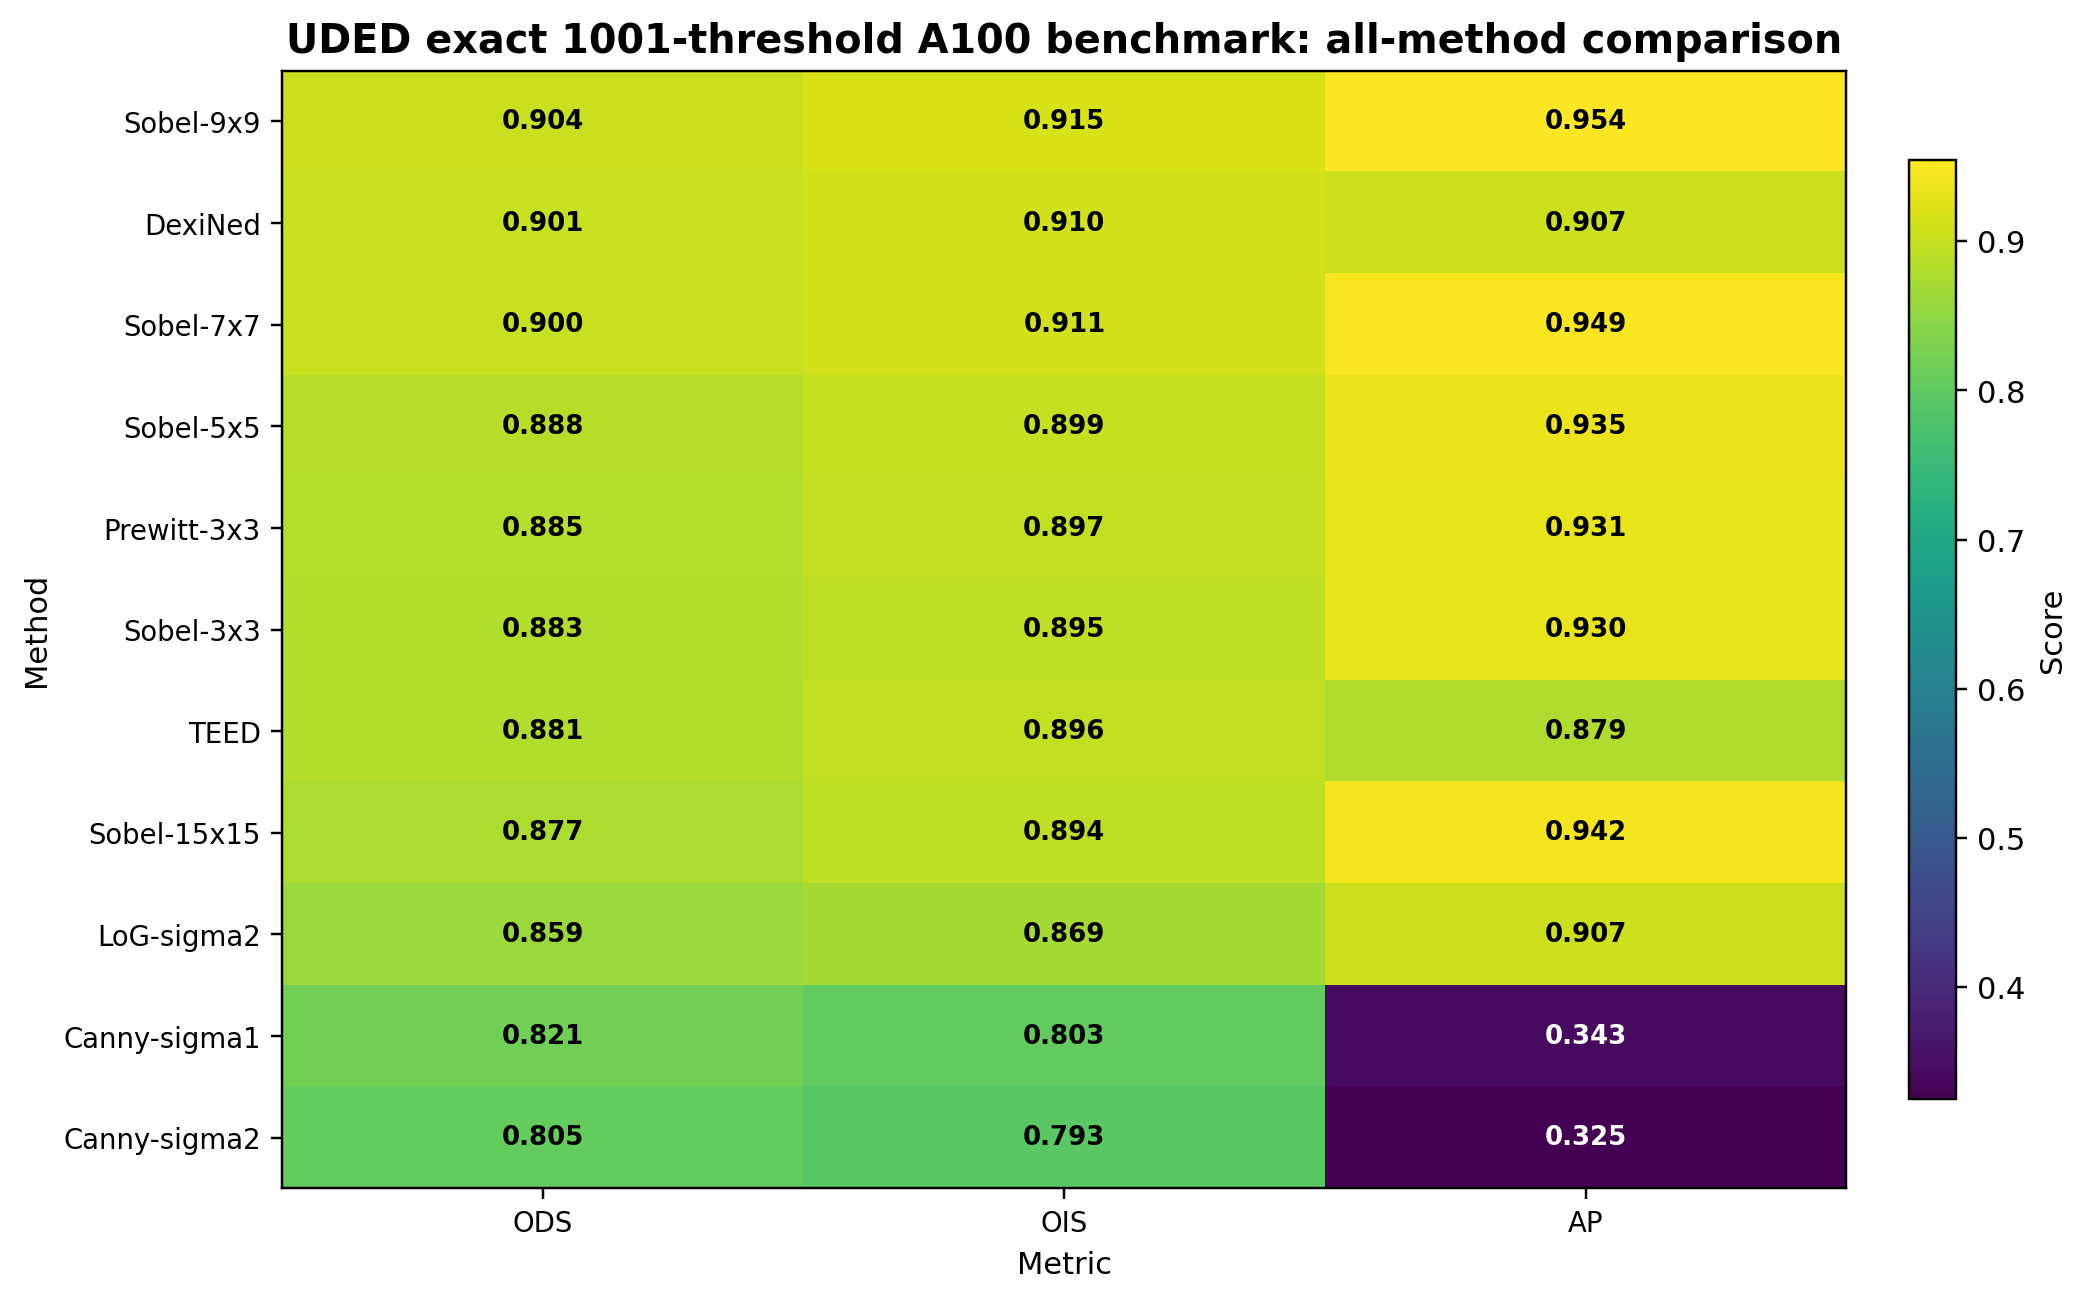
\includegraphics[width=0.93\textwidth]{figures/uded_metric_heatmap.png}
  \caption{Exact UDED A100 benchmark summary from the local JSON artifact. The heatmap compares ODS, OIS, and AP across all reproduced methods. The result is intentionally compact: the best overall method is a classical large-support Sobel filter, not a learned detector.}
  \label{fig:heatmap}
\end{figure*}

\begin{table*}[t]
  \centering
  \footnotesize
  \setlength{\tabcolsep}{4.5pt}
  \renewcommand{\arraystretch}{1.15}
  \caption{Exact UDED 1001-threshold A100 benchmark. Learned methods use PyTorch inference on CUDA when available; classical methods run in NumPy/SciPy. The benchmark used 30 images, a 3-pixel match radius, and all 1001 thresholds.}
  \label{tab:metrics}
  \begin{tabular}{l l c c c c}
    \toprule
    Method & Type & ODS & OIS & AP & Time (ms/img) \\
    \midrule
    Sobel-9$\times$9  & traditional & 0.9039 & 0.9151 & 0.9543 & 26.2 \\
    DexiNed           & ml          & 0.9010 & 0.9102 & 0.9068 & 215.3 \\
    Sobel-7$\times$7  & traditional & 0.9004 & 0.9109 & 0.9489 & 22.7 \\
    Sobel-5$\times$5  & traditional & 0.8877 & 0.8987 & 0.9351 & 25.6 \\
    Prewitt-3$\times$3& traditional & 0.8848 & 0.8972 & 0.9314 & 31.0 \\
    Sobel-3$\times$3  & traditional & 0.8828 & 0.8951 & 0.9299 & 28.9 \\
    TEED              & ml          & 0.8814 & 0.8958 & 0.8787 & 210.1 \\
    Sobel-15$\times$15& traditional & 0.8770 & 0.8939 & 0.9425 & 34.7 \\
    LoG-$\sigma$2     & traditional & 0.8587 & 0.8689 & 0.9073 & 661.6 \\
    Canny-$\sigma$1   & traditional & 0.8211 & 0.8034 & 0.3428 & 90.4 \\
    Canny-$\sigma$2   & traditional & 0.8047 & 0.7927 & 0.3252 & 55.6 \\
    \bottomrule
  \end{tabular}
\end{table*}

The near-tie between Sobel-9$\times$9 and DexiNed is real, but it should not be overstated. Sobel-9$\times$9 leads DexiNed by 0.0029 ODS points and 0.0049 OIS points, which is small enough to call a near-tie. The AP difference is much larger: Sobel-9$\times$9 exceeds DexiNed by about 0.0475 AP points. That means the classical baseline is not just matching the learned model at a single operating point; it is also accumulating more area under the precision-recall curve across the threshold sweep.

\subsection{Runtime and efficiency}
Figure~\ref{fig:runtime} shows the runtime ranking from the same benchmark. DexiNed is about 8.2$\times$ slower than Sobel-9$\times$9 in the benchmark pipeline, and TEED is similarly slow. Because the benchmark mixes CPU classical filters with GPU-capable learned models, the runtime comparison is not a pure apples-to-apples hardware comparison; however, it is still operationally meaningful. Even with CUDA available to the learned models, the classical large-support Sobel filters remain much faster in this run.

\begin{figure*}[t]
  \centering
  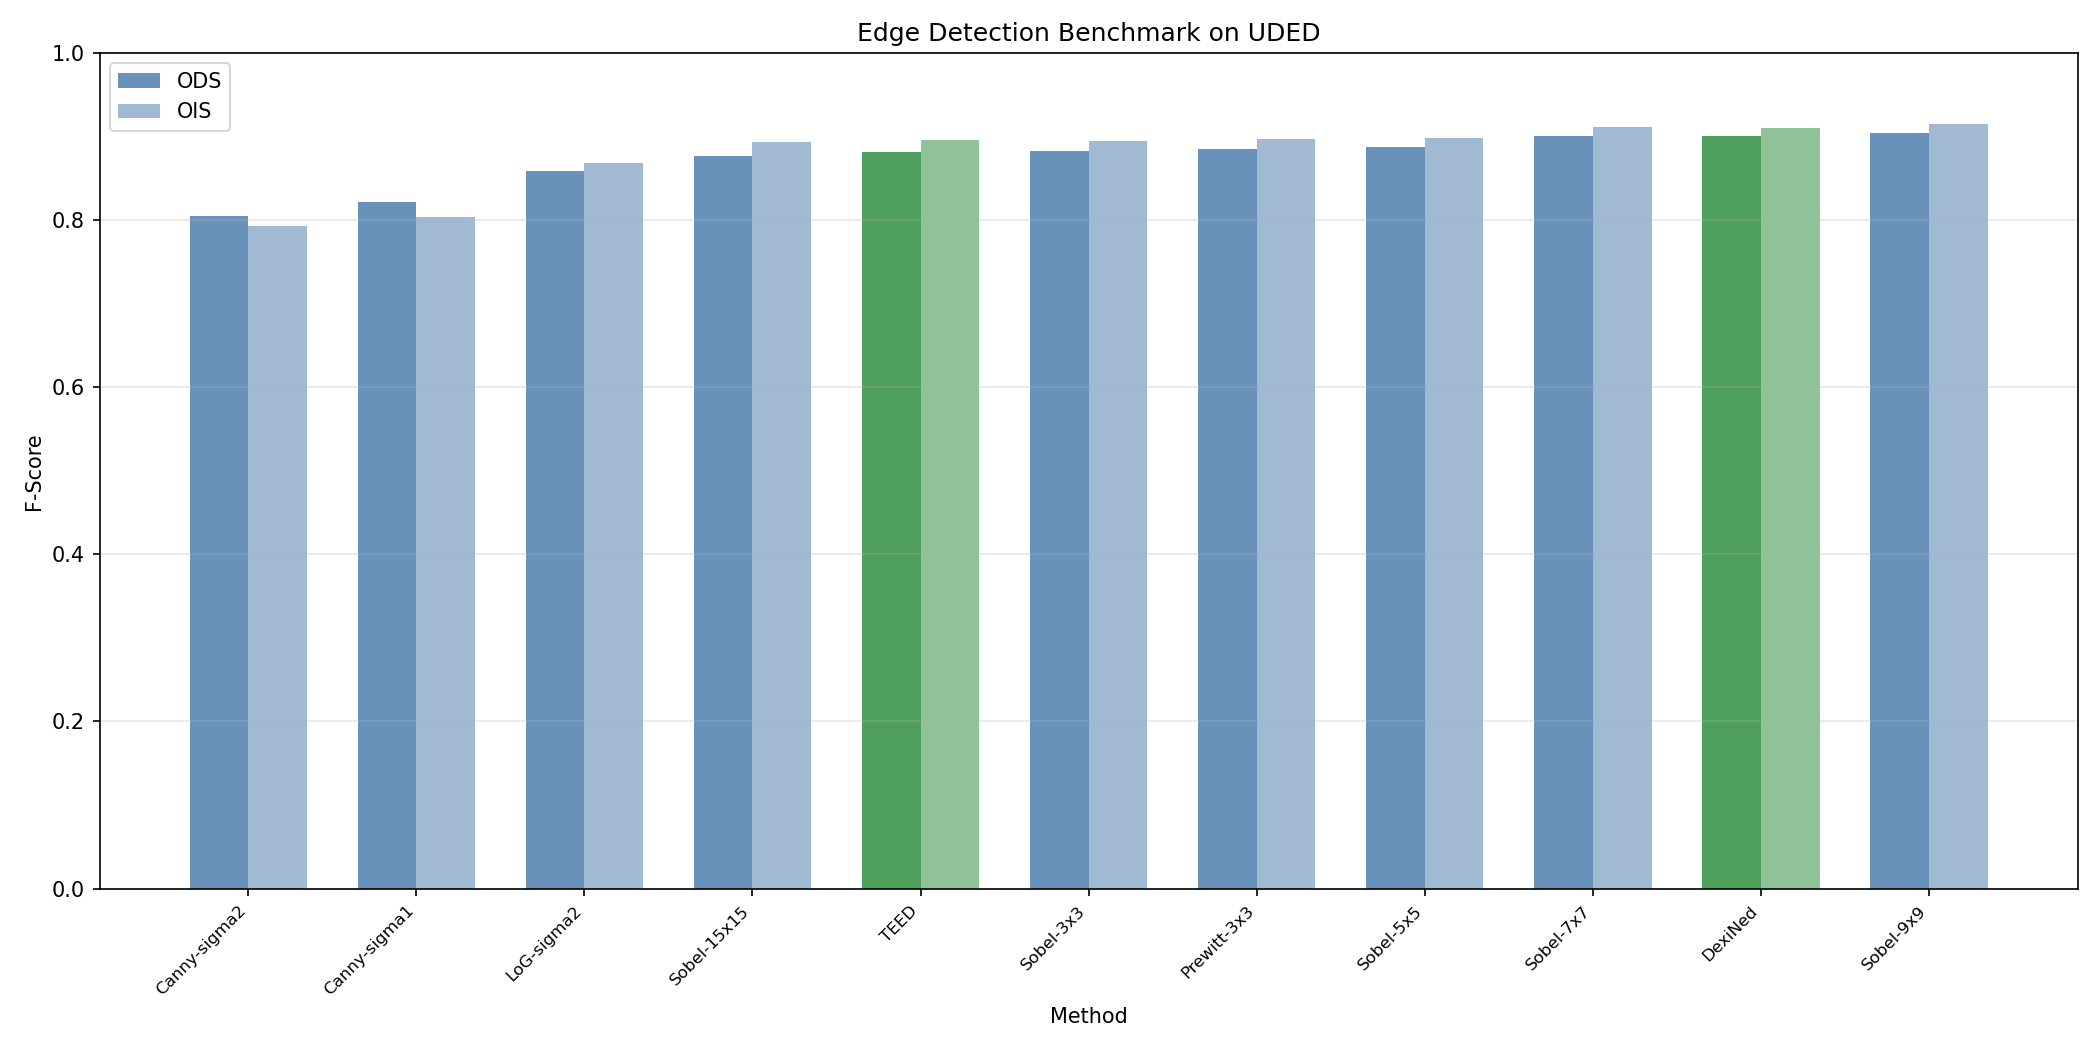
\includegraphics[width=0.93\textwidth]{UDED_exact1001_uded_a100_ods_ois.png}
  \caption{Exact UDED ODS/OIS comparison from the local benchmark report. The salient feature is the near-tie between Sobel-9$\times$9 and DexiNed at the top of the ranking, with large-support Sobel still slightly ahead.}
  \label{fig:ods_ois}
\end{figure*}

\begin{figure*}[t]
  \centering
  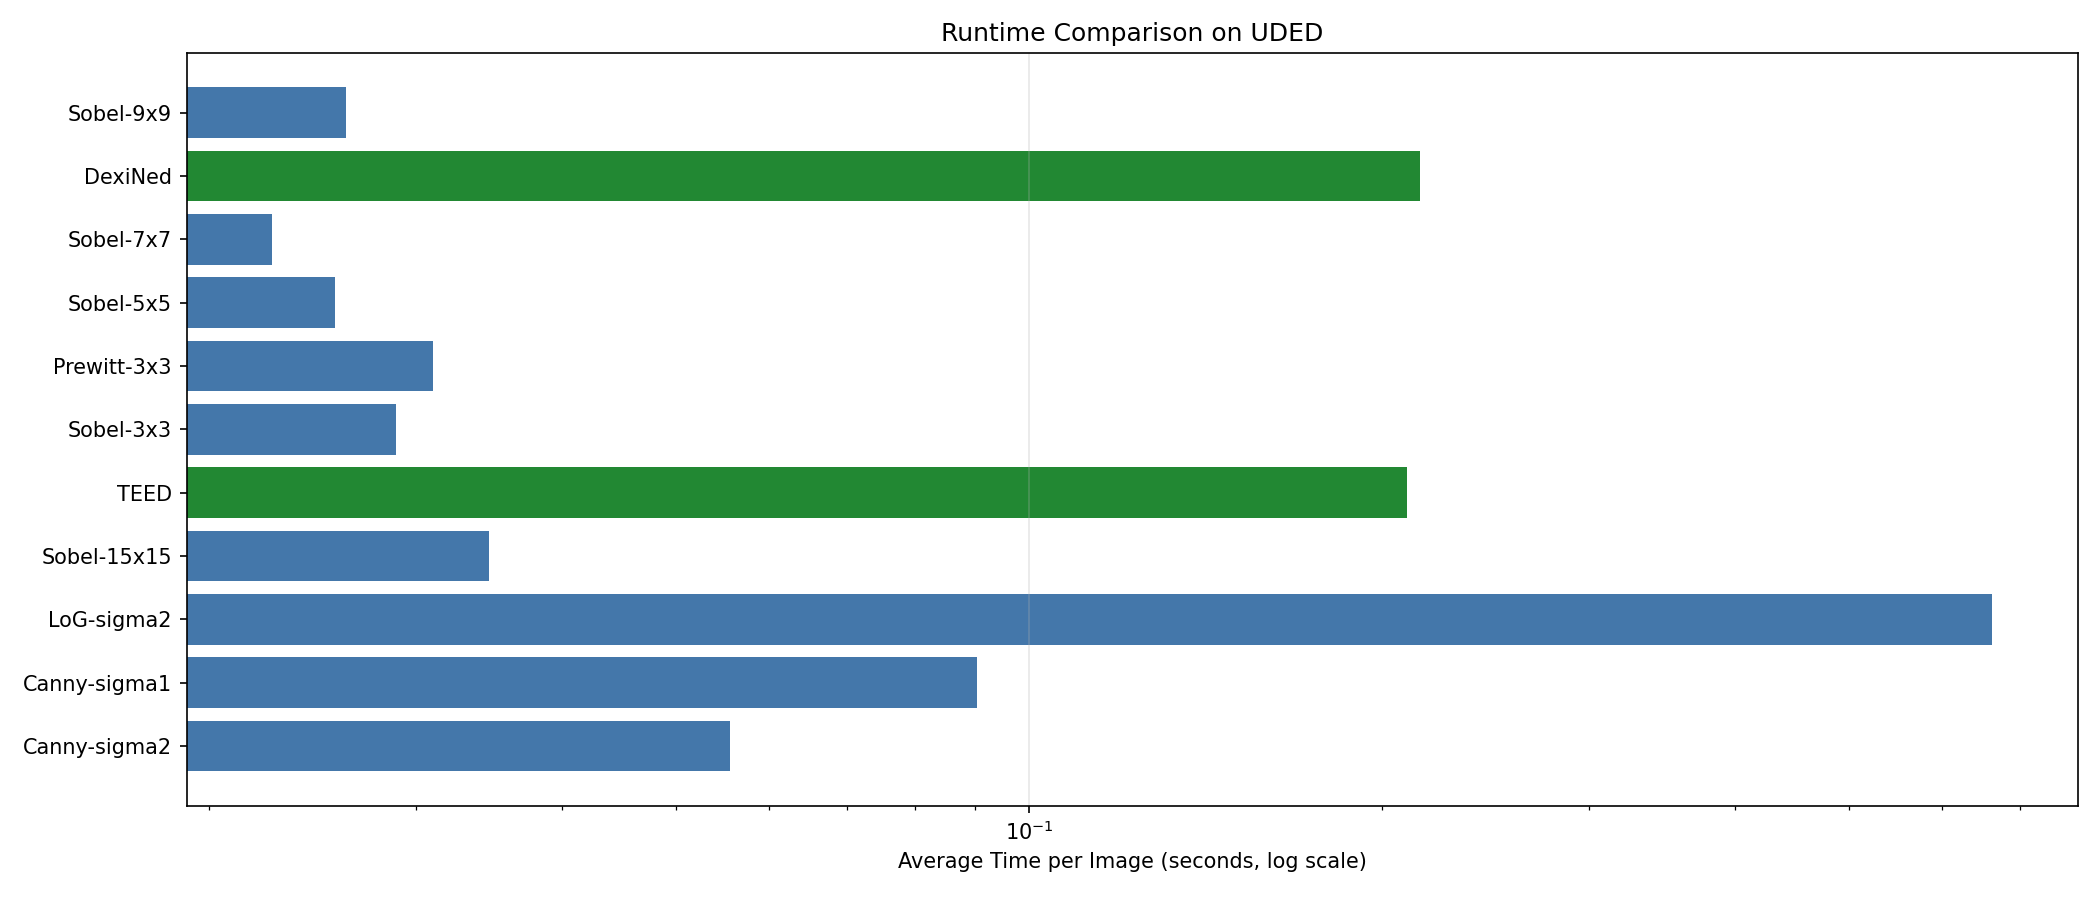
\includegraphics[width=0.93\textwidth]{UDED_exact1001_uded_a100_runtime.png}
  \caption{Exact UDED runtime comparison from the local benchmark report. The learned methods are much slower in the measured pipeline, even though CUDA was available for PyTorch inference.}
  \label{fig:runtime}
\end{figure*}

The runtime gap matters because the source framing often treats learned detectors as if they were the only plausible route to good generalization. This benchmark says something less dramatic but more useful: a carefully chosen classical support size can be competitive in accuracy while remaining dramatically cheaper in this local evaluation pipeline. If the deployment question is edge detection under limited compute, that tradeoff is hard to ignore.

\subsection{What the AP gap changes}
The AP gap is the most informative part of the result. ODS and OIS are thresholded summary scores, so a near-tie there can hide the shape of the precision-recall curve. AP exposes that shape. The fact that Sobel-9$\times$9 wins AP by a comfortable margin means the classical baseline is not merely benefiting from a favorable single threshold. It is stable over the sweep. That is a stronger result than the ODS tie alone would suggest.

This also changes how the result should be read against the source papers. If a paper claims that a new method is superior because it looks better visually or because it wins at one operating point, the exact UDED benchmark shows why that argument is incomplete. A single threshold or a coarse sweep can miss that a classical method has broader threshold robustness.

\section{Implications for Aquatic-Domain Claims}
The main implication is not that aquatic-domain claims are false. The implication is that the local UDED evidence does not support a broad claim of modern learned superiority. UDED is a general edge benchmark, not the aquatic hand-labeled test set emphasized in the WVF/LF thesis and OCEANS papers. So this benchmark cannot by itself validate the aquatic-specific parts of the source story. What it \emph{can} do is audit the generalization claim that UDED is often used to support.

On that narrower question, the answer is unfavorable to a simple ``CNNs beat classical filters'' narrative. Sobel-9$\times$9 is the best reproduced method on UDED under the exact protocol. DexiNed is close, but not better. TEED trails both. If the source papers use UDED as part of a broader argument that their aquatic-domain methods are competitive or superior to other detectors, this exact result should force a more careful statement: the evidence is method- and protocol-sensitive, and UDED alone does not establish a universal ranking.

The result is also a reminder that baseline choice matters. If the comparison set is only $3{\times}3$ operators, the story looks much weaker than if large-support Sobel and related classical filters are included. That is relevant to the thesis and OCEANS line of work because their narrative benefits from comparing against genuinely strong classical alternatives, not only minimal-support edge operators.

\section{What Remains Untested}
This paper intentionally stops short of claiming a full reproduction of the WVF/LF aquatic pipeline. Several important pieces remain untested locally:
\begin{itemize}
  \item WVF and LF are not re-evaluated here on exact UDED settings from the source papers.
  \item The local repository does not contain the four-image hand-labeled aquatic set described in the thesis and OCEANS papers.
  \item \texttt{datasets/BIPED} is not populated in the current workspace, so the BIPED tables and visual comparisons remain out of reach.
  \item The multi-scale and multi-domain orientation pipeline from the later OCEANS paper is not reproduced here.
\end{itemize}

Those gaps matter because they delimit the claims this paper can make. The local exact UDED run is strong evidence against an overconfident generalization story, but it is not a definitive verdict on the full WVF/LF family in its intended aquatic regime.

\section{Conclusion}
The exact 1001-threshold A100 benchmark on UDED is the most reliable piece of evidence currently available in this workspace for judging the general edge-detection claims. Its message is not subtle: Sobel-9$\times$9 is the best reproduced method, DexiNed is close on ODS/OIS but weaker on AP, and the learned models are far slower in the benchmark pipeline. That combination undercuts any easy claim that modern learned detectors clearly dominate classical filters on UDED.

For aquatic-domain claims, the conclusion is narrower but still important. UDED does not directly test the source papers' aquatic dataset, and this paper does not pretend otherwise. What it does show is that the source-paper framing should be tightened: UDED supports a claim about careful benchmarking and parameter sensitivity, not a blanket claim of learned superiority.

\begin{thebibliography}{99}

\bibitem{udedrepo}
X.~Soria \emph{et al.}, ``UDED: Unified Dataset for Edge Detection,'' GitHub repository. [Online]. Available: \url{https://github.com/xavysp/UDED}

\bibitem{teed2023}
X.~Soria, Y.~Li, M.~Rouhani, and A.~D.~Sappa, ``Tiny and Efficient Model for the Edge Detection Generalization,'' in \emph{Proc. IEEE/CVF Int. Conf. Comput. Vis. Workshops (ICCVW)}, 2023, pp.~1364--1373.

\bibitem{dexined2023}
X.~Soria, A.~Sappa, P.~Humanante, and A.~Akbarinia, ``Dense Extreme Inception Network for Edge Detection,'' \emph{Pattern Recognition}, vol.~139, p.~109461, 2023.

\bibitem{bagan_thesis}
Bagan, \emph{Wide View and Line Filter for Enhanced Image Gradient Computation}, M.S. thesis, Univ. of South Carolina, 2023.

\bibitem{bagan_2024}
Bagan and Wang, ``Wide View and Line Filter for Enhanced Gradient Computation in Aquatic Environment,'' in \emph{Proc. IEEE OCEANS Great Lakes}, 2024, pp.~1--10.

\bibitem{bagan_2025}
Bagan and Wang, ``Multi-Scale and Multi-Domain Edge Determination with Accurate Gradient Orientation Computation in Aquatic Environment,'' in \emph{Proc. IEEE OCEANS Great Lakes}, 2025, pp.~1--9.

\end{thebibliography}

\end{document}
